% Faculty-facing course report. Supporting records preserve numerical provenance.
% The layout and section order follow the supplied course template.
\documentclass[10pt]{article}
\usepackage[margin=0.72in]{geometry}
\usepackage[T1]{fontenc}
\usepackage{lmodern}
\usepackage{microtype}
\usepackage{booktabs}
\usepackage{graphicx}
\usepackage{amsmath,amssymb}
\usepackage{xcolor}
\usepackage{hyperref}
\usepackage{enumitem}
\definecolor{hkustblue}{HTML}{003B71}
\hypersetup{colorlinks=true,urlcolor=hkustblue,citecolor=hkustblue}
\setlength{\parindent}{0pt}
\setlength{\parskip}{4pt}

\title{\vspace{-1.5em}\textbf{Context, Not Grammar?}\\
Where Transformers Beat LSTMs in Small-Scale Language Modeling}
\author{Cao Pham Minh Dang (21453430) \and Hugo Centeno Sanz}
\date{COMP 4221 Natural Language Processing --- Fall 2026}

\begin{document}
\maketitle

\begin{abstract}
Better text prediction does not necessarily imply better grammatical knowledge. We hypothesize that Transformer attention improves the use of preceding context, rather than grammatical discrimination, compared with classic long short-term memory (LSTM) networks, and we will test this using matched training, context interventions, repeated-text prediction, and grammatical minimal pairs. We trained both model families on WikiText-103 with one shared tokenizer, approximately 7.5, 17.1, or 50.2 million parameters, 250 million predicted tokens per run, and three independent training repetitions at each size. Transformer test perplexities are 40.31, 30.75, and 24.70 for the small, medium, and large models, compared with 56.58, 44.57, and 42.55 for LSTMs; lower values indicate better prediction. Transformers benefit more from repeated text and lose more predictive accuracy when distant context is removed while the predicted tokens remain fixed. Grammar results differ: the accuracy gap changes direction across sizes, and no comparison establishes equivalence within the prespecified two-percentage-point margin. A 5-gram baseline is unaffected by changes beyond its four-token history, confirming that the context intervention distinguishes finite from longer-range memory. A deeper LSTM does not close the observed gap, although one training repetition fails. The evidence supports stronger contextual prediction by Transformers under these conditions, but does not establish grammar equivalence or show that distant context explains most of the perplexity advantage.
\end{abstract}

\section{Introduction}

Lower prediction loss can reflect local grammar, retrieval of earlier words, or sequence repetition. Perplexity summarizes how uncertain a language model is about the next token; it combines these abilities and cannot establish which improved. This distinction matters when comparing Transformers, which attend directly to preceding token representations, with classic long short-term memory (LSTM) networks, which compress preceding information into a recurrent state.

Both families learn from the same WikiText-103 articles and tokenizer. Training examples are independent text segments containing at most 512 tokens to predict. We compare small, medium, and large models, with approximately 7.5, 17.1, and 50.2 million parameters. At each size, the two families share embedding widths and closely matched counts of other parameters. Each model predicts 250 million training tokens, and each configuration is trained three times with different random seeds, the numerical settings that control initialization and data order. These repetitions reveal variation caused by training rather than by the choice of test examples.

We test three predictions. The \textbf{context and copying hypothesis} predicts larger reductions in prediction loss at later text positions and on repeated passages for Transformers. The \textbf{grammar-equivalence hypothesis} predicts that overall grammatical judgment accuracy differs by less than two percentage points. The \textbf{scaling hypothesis} predicts that the context advantage grows with model size while the grammar gap remains small. To test context use directly, we also predict identical tokens after shortening or shuffling their preceding text. This separates the effect of available history from differences in the difficulty of tokens at early and late positions.

Our contribution is a controlled account of which advantages appear under this budget. Transformer context and repetition scores consistently exceed LSTM scores, while grammar gaps change direction across sizes. Stronger position-wise gains at larger sizes do not imply steadily larger benefits from context beyond 128 tokens. These controls qualify the context-use interpretation rather than establish universal attention superiority.

\section{Related Work}

Transformer attention~\cite{vaswani2017attention} and LSTM gated recurrence~\cite{hochreiter1997lstm} offer different routes to preceding information. Kaplan et al.~\cite{kaplan2020scaling} relate performance to size, data, and compute, motivating our context-position and size comparisons. Our small fixed-budget experiment does not establish a general scaling law.

Khandelwal et al.~\cite{khandelwal2018context} distinguish the precise use of nearby words from more approximate use of distant context in recurrent language models. Olsson et al.~\cite{olsson2022induction} connect repeated-pattern completion in attention models with induction mechanisms. These motivate our history interventions and copy tasks, but behavioral copy gains alone do not identify an internal circuit. Patil et al.~\cite{patil2024fict} further motivate evaluating linguistic generalization separately from aggregate language-model loss.

WikiText provides article-level text suitable for studying contextual prediction~\cite{merity2017pointer}. The Benchmark of Linguistic Minimal Pairs (BLiMP) tests grammatical contrasts using pairs of minimally different sentences~\cite{warstadt2020blimp}, although scoring depends on tokenization and candidate length~\cite{ueda2024length}. We retain summed log probability as the primary grammar score and examine length-based alternatives separately. KenLM~\cite{heafield2011kenlm} supplies a 5-gram baseline whose predictions depend on at most four preceding tokens. It should therefore remain exactly unchanged when only more distant context is altered.

\section{Data and Task Formulation}

We use the raw-text version of WikiText-103 and retain its official training, validation, and test splits. Article reconstruction preserves source text and article order rather than treating every input row as a separate document. The splits contain 28,472, 60, and 60 articles, respectively. Dataset versions and file checksums are recorded for reproducibility. One identical article occurs in both training and test data; it is retained to preserve the official splits and limits claims about entirely novel test content.

A shared tokenizer uses byte-level byte-pair encoding (BPE)~\cite{sennrich2016subword}, learned from the training articles only. It represents text with 16,384 token types, including symbols for padding, beginning of sequence (BOS), end of sequence (EOS), and unknown text. Byte coverage preserves case, whitespace, and Unicode without normalization; encoding and decoding recover every WikiText article exactly. Both neural families and the 5-gram model use these same tokens, making losses directly comparable. KenLM treats each token as a word symbol and each article ending as a sentence boundary.

Each article contributes one end token. Nonoverlapping segments, subsequently called context windows, contain up to 512 tokens to predict and never cross article boundaries. For target tokens $z_1,\ldots,z_T$, the input is $[\mathrm{BOS},z_1,\ldots,z_{T-1}]$. Padding does not contribute to loss, and both Transformer positions and LSTM memory states restart in every window. Training, validation, and test contain 122,022,510, 255,099, and 291,710 prediction targets in 252,574, 529, and 602 windows. Test perplexity includes all windows. Position curves and context interventions use the 542 complete test windows, excluding 60 shorter windows and 14,206 targets.

Grammar evaluation uses all 67,000 BLiMP pairs across 67 grammatical contrasts and 12 phenomenon groups. A pair is correct only when the grammatical sentence receives a strictly larger probability; ties count as incorrect. BLiMP is used only for final evaluation, never to select training settings or saved model weights. WikiText's metadata and description disagree about the CC BY-SA license version (3.0/GFDL versus 4.0); the attribution record preserves that discrepancy. BLiMP lists CC BY 4.0. Public text can contain social biases and personal information, so public availability does not imply suitability for unrestricted generation or decisions about people.

\section{Approach}

\subsection{Matched language models}

We implemented data preparation, tokenizer training, neural models, training, and evaluation using PyTorch and Hugging Face Tokenizers; 5-gram estimation uses KenLM. The causal Transformer uses pre-normalized residual blocks, multihead self-attention, learned absolute positions, and a feedforward network with a Gaussian error linear unit activation and width $4d$, where $d$ is the token embedding dimension. The LSTM has two standard recurrent layers of hidden width $h$. A linear $h\!\rightarrow\!d$ adapter maps recurrent outputs back to the embedding dimension. Both families reuse their input embedding matrix to predict output tokens. Table~\ref{tab:parameters} reports actual parameter counts, including the adapter and positional embeddings. Counts excluding token embeddings differ by at most 0.16\%, within the prespecified 5\% tolerance; exact counts appear in Table~\ref{tab:exactcounts}.

\begin{table}[t]
\centering
\small
\begin{tabular}{lrrrrrr}
\toprule
Size & $d$ & \shortstack{Attention\\layers/heads} & \shortstack{Recurrent\\layers/$h$} & \shortstack{Transformer\\parameters} & \shortstack{LSTM\\parameters} & \shortstack{Other parameter\\difference} \\
\midrule
Small & 256 & 4 / 4 & 2 / 472 & 7,484,928 & 7,479,680 & $-0.16\%$ \\
Medium & 384 & 6 / 6 & 2 / 873 & 17,135,616 & 17,127,516 & $-0.07\%$ \\
Large & 640 & 8 / 10 & 2 / 1690 & 50,202,880 & 50,194,640 & $-0.02\%$ \\
Medium, deeper & 384 & 6 / 6 & 4 / 588 & 17,135,616 & 17,120,448 & $-0.14\%$ \\
\bottomrule
\end{tabular}
\caption{Architectural dimensions and total parameter counts. The final column compares LSTM and Transformer parameters excluding token embeddings, relative to the Transformer count. Shared input/output embeddings are counted once. The four-layer medium LSTM is a separate depth control.}
\label{tab:parameters}
\end{table}

Both neural families minimize next-token negative log likelihood (NLL), using the true preceding tokens during training. Let $i$ identify a window, $t$ a target position, $m_{it}$ indicate a nonpadding target, and $p_\theta$ be the model's predicted probability. The average loss and perplexity are
\begin{equation}
\mathcal{L}=-\frac{\sum_{i,t}m_{it}\log p_\theta(z_{it}\mid z_{i,<t})}{\sum_{i,t}m_{it}},
\qquad \mathrm{Perplexity}=\exp(\mathcal{L}).
\label{eq:loss}
\end{equation}
Loss is measured in nats, the units obtained with natural logarithms; lower loss and perplexity mean better prediction. We sum losses and target counts before dividing. KenLM uses unpruned interpolated modified Kneser--Ney smoothing on the same training text. It starts evaluation windows without a special article-start history, because most windows begin inside an article. Its base-10 log probabilities are converted to natural logarithms.

\subsection{Context, copying, and grammar}

Our first context measure is \emph{context gain}: the difference between average prediction loss near the beginning and near the end of a complete window,
\begin{equation}
\text{Context gain}=\frac{1}{32}\sum_{t=1}^{32}\bar\ell(t)
-\frac{1}{128}\sum_{t=385}^{512}\bar\ell(t),
\label{eq:cg}
\end{equation}
where $\bar\ell(t)$ is average loss at position $t$. A positive value indicates better prediction at later positions, when more context is available. However, later tokens may also be intrinsically easier to predict, so this measure alone does not establish a benefit from longer context.

To address that ambiguity, the context intervention holds fixed all 69,376 targets at positions 385--512 of complete test windows. Each target is predicted from its full preceding context, only its nearest $k\in\{4,32,128\}$ tokens, or a full-length context in which tokens beyond the nearest 128 are shuffled. Each input begins with a sequence-start symbol and fresh model state. The truncation penalty is
\begin{equation}
G_k=\frac1N\sum_{j=1}^N\bigl[\ell_j(k)-\ell_j(\mathrm{full})\bigr],
\label{eq:intervention}
\end{equation}
where $N$ is the number of targets and $\ell_j(k)$ is target $j$'s loss with only $k$ preceding tokens. A positive penalty means that the removed history helped prediction. We calculate an analogous penalty for shuffling. Truncation also changes positions and the number of recurrent updates before prediction. Shuffling preserves these features, although rearranging subword tokens disrupts word forms as well as distant order. The two tests therefore provide complementary evidence rather than a pure separation of semantic effects.

The repetition task presents a token sequence $A$ followed by an exact copy of $A$. Repetition gain is the first occurrence's average loss minus the second's, for a sequence of length $L$. We use lengths 25, 50, 100, and 200, sampling 1,000 examples per length from natural test text and from uniformly sampled ordinary tokens. The main endpoint is natural-text repetition of length 100. Controls replace the repeated sequence with an independently sampled sequence and exclude each sequence's first four positions. Although sampling rules agree, the Transformer and baseline evaluations used different sampled sequences; their differences are therefore descriptive comparisons, not comparisons of identical test examples.

For each BLiMP sentence, we sum subword log probabilities from the sequence-start symbol through the end symbol. The model succeeds when the grammatical sentence has the larger sum. We separately examine pairs with equal token counts and scores averaged per token to assess sensitivity to sentence length.

\section{Experimental Setup}

The main experiment comprises 18 training runs: two architectures, three model sizes, and three random seeds (13, 37, and 73). Each run predicts exactly 250 million nonpadding tokens, including article endings. Corresponding runs use the same rule for shuffling training windows. Training uses 32-bit floating-point arithmetic and batches of 64 windows, processed in four groups of 16 before each parameter update. Both families use AdamW with $(\beta_1,\beta_2)=(0.9,0.95)$, weight decay 0.1 except on biases and normalization parameters, gradient clipping at norm 1, and a cosine learning-rate schedule with 1\% warm-up. Loss normalization and the final partial batch count only the actual prediction targets.

Hyperparameters are selected using the small model of each family. The initial eight-setting search was expanded equally for both families to six learning rates ($10^{-4},3\!\times\!10^{-4},10^{-3},3\!\times\!10^{-3},10^{-2},3\!\times\!10^{-2}$) and dropout probabilities 0 or 0.1. Each of the resulting 12 trials predicts 50 million tokens with a separate tuning seed, 101. Validation loss selects learning rate 0.001 and no dropout for Transformers, and learning rate 0.03 with dropout 0.1 for LSTMs. These settings transfer unchanged to medium and large models and to the deeper LSTM control. Equal searches avoid extra tuning for favorable larger models, but do not guarantee equally suitable settings at every size.

Model weights are saved and evaluated on validation text approximately every million training tokens, as well as before and after training. The main results use the saved version with the lowest validation loss from each run. Weights at the end of training provide a separate comparison. Neither test text nor grammar scores influence model selection. Preliminary runs and separate batch-size experiments are excluded from the main statistical analysis.

One initialization choice differs between families. LSTM token embeddings are sampled uniformly from $[-0.1,0.1]$, after smaller normally distributed embeddings produced prolonged training stagnation. Transformer matrices retain normal initialization with standard deviation 0.02. This change preceded the final hyperparameter search. The comparison consequently evaluates two documented training procedures rather than changing architecture while holding every numerical choice identical.

Training uses university GPUs. Transformer runs use 24-GB RTX 3090 devices and average 0.51, 1.00, and 2.26 hours of parameter-update time for small, medium, and large models, totaling 11.29 GPU-hours across nine runs. Validation and saving weights add overhead. LSTM runs average 0.61, 0.55, and 1.67 hours on an RTX 4090 D; different hardware prevents an architectural speed comparison. Estimated Transformer matrix computation is $1.33\times10^{16}$, $3.06\times10^{16}$, and $8.75\times10^{16}$ floating-point operations per run. These estimates approximate backward computation as twice forward computation and exclude normalization, nonlinearities, and optimizer work. Token exposure is matched; computation is not. The four-layer medium LSTM fails for seed 37 at learning rate 0.03. A separate three-seed test uses learning rate 0.01 and no dropout, without replacing the failed run.

Statistical comparisons use independently trained models as the replication units, pairing runs by random seed. We report sample standard deviations and 95\% Student-$t$ intervals for differences between architectures, assuming approximately normal seed-level differences. These three-run estimates differ from uncertainty obtained by resampling test examples for a fixed model. Holm correction accounts for the planned multiple comparisons: six context/repetition tests across three sizes, three grammar-equivalence tests, and two scaling tests. Because repetition evaluations used different examples, their confirmatory tests are withheld; conservative values of 1 are used only in the multiplicity adjustment to preserve the original comparison counts. Grammar equivalence requires two one-sided tests (TOST) against a fixed margin of two percentage points. A nonsignificant conventional difference test does not establish equivalence.

\section{Results}

\begin{table}[t]
\centering
\small
\begin{tabular}{llrrrrr}
\toprule
Model & Size & \shortstack{Test\\perplexity $\downarrow$} & \shortstack{Grammar\\accuracy (\%) $\uparrow$} & \shortstack{Context\\gain $\uparrow$} & \shortstack{Repetition\\gain $\uparrow$} & \shortstack{128-token\\penalty $\uparrow$} \\
\midrule
Transformer & Small & 40.31 & 59.58 & 0.639 & 1.298 & 0.093 \\
LSTM & Small & 56.58 & 62.23 & 0.400 & 0.068 & 0.014 \\
Transformer & Medium & 30.75 & 61.49 & 0.692 & 1.553 & 0.098 \\
LSTM & Medium & 44.57 & 62.97 & 0.441 & 0.096 & 0.018 \\
Transformer & Large & 24.70 & 63.97 & 0.713 & 1.626 & 0.097 \\
LSTM & Large & 42.55 & 62.12 & 0.436 & 0.090 & 0.018 \\
\midrule
KenLM 5-gram & -- & 66.45 & 54.00 & 0.183 & $-0.024$ & 0.000 \\
\bottomrule
\end{tabular}
\caption{Results for models selected by validation loss, averaged across three training repetitions. Grammar accuracy uses BLiMP. Repetition gain uses 100-token natural-text sequences. The 128-token penalty measures the loss increase after removing more distant history. Gains and penalties are in nats per token. Repetition examples differ between architectures. Perplexity is averaged over runs; the 5-gram model is one deterministic baseline.}
\label{tab:main}
\end{table}

Transformers predict held-out text better at every size (Table~\ref{tab:main}, Figure~\ref{fig:architecture}). Their perplexity reductions relative to LSTMs are approximately 29\%, 31\%, and 42\% for small, medium, and large models. Both families outperform the 5-gram baseline. LSTM perplexity improves strongly from small to medium but only modestly, on average, from medium to large, with substantial variation between large-model runs. Transformer improvements are more consistent across sizes. These are comparisons at equal training-token exposure, not equal computation.

\textbf{Context and copying hypothesis.} Transformer context gain exceeds LSTM context gain by 0.239, 0.251, and 0.277 nats for small, medium, and large models. The 95\% intervals exclude zero, and corrected one-sided tests remain significant ($p=0.0130,0.00073,0.0130$). Natural-text repetition gains are also much larger: 1.30--1.63 nats for Transformers versus 0.07--0.10 for LSTMs. Holding the predicted tokens fixed strengthens the context interpretation: limiting history to 128 tokens increases Transformer loss by about 0.09--0.10 nats, compared with 0.01--0.02 for LSTMs. The evidence supports the context-gain prediction and corroborates stronger repetition behavior. Because the repetition tests used different sampled sequences, their observed separation remains descriptive rather than a confirmation based on identical examples.

\textbf{Grammar-equivalence hypothesis.} The Transformer minus LSTM accuracy gap changes direction: $-2.65$, $-1.48$, and $+1.85$ percentage points for small, medium, and large models. Better text prediction therefore does not guarantee better grammatical judgments. The small-model mean lies outside the two-point equivalence margin. For medium and large models, means inside the margin are insufficient because training variation must also be considered. No size passes the equivalence test: unadjusted $p=0.705,0.319,0.428$, with corrected $p=0.956$ for all three. The corresponding 90\% intervals are $[-5.64,0.34]$, $[-4.25,1.29]$, and $[-0.34,4.03]$ percentage points. Each extends beyond an equivalence boundary. Grammar equivalence is therefore inconclusive.

\textbf{Scaling hypothesis.} Better absolute scores at larger sizes do not establish that the \emph{difference between architectures} grows reliably. The context-gain gap increases from 0.239 to 0.277 nats between the smallest and largest models, a change of only 0.038 nats (95\% interval $[-0.115,0.191]$, corrected $p=0.396$). The repetition-gap change is 0.306 nats, with a descriptive interval of $[-0.345,0.956]$ conditional on the different test samples. Neither provides clear evidence of increasing advantage. Transformer benefits from history beyond 128 tokens are also nearly flat across sizes. The scaling hypothesis is not statistically supported.

\begin{figure}[t]
\centering
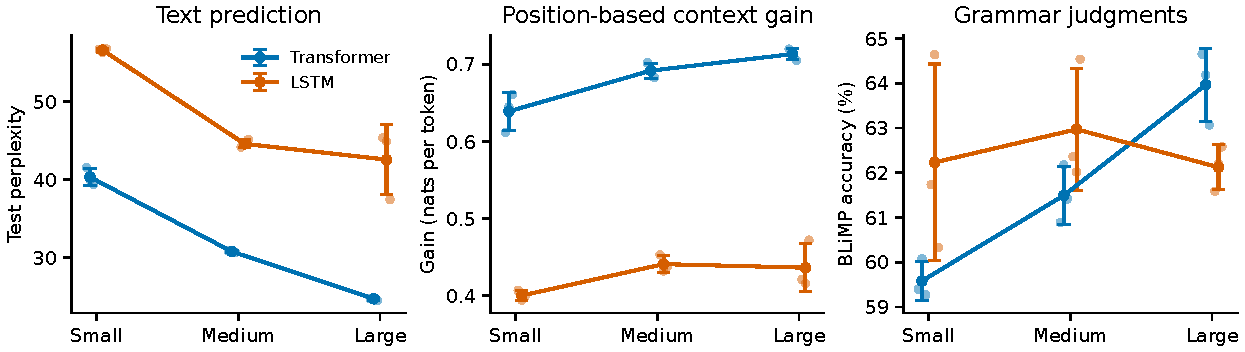
\includegraphics[width=0.96\linewidth]{figures/architecture_comparison.pdf}
\caption{Prediction, context gain, and grammar accuracy across small, medium, and large models. Small dots represent independent training repetitions; error bars show sample standard deviations rather than confidence intervals. Grammar equivalence is tested on paired differences, not on the absolute accuracies plotted here.}
\label{fig:architecture}
\end{figure}

\section{Analysis}

\subsection{Why controlling the predicted tokens changes the interpretation}

The 5-gram baseline has a positive context gain of 0.183 nats despite being unable to use more than four preceding tokens. Its largest losses occur at the beginning of a window, where even that short history is incomplete. A positive early-to-late improvement is therefore insufficient evidence of long-context use. Beyond each repeated sequence's first four positions, its repetition gain is exactly zero. Its predictions also remain exactly unchanged under every context truncation and distant shuffle tested here. These expected properties validate the scoring procedure and explain the baseline's role.

The neural interventions ask a more controlled question: does preceding text help predict a fixed set of tokens? Transformers suffer much larger losses than LSTMs when those tokens lose most of their history. The effect persists with 128 preceding tokens retained; shuffling more distant text also hurts prediction while preserving input length and the local context (Figure~\ref{fig:context}). Together these results indicate that Transformers use information that classic LSTMs preserve less effectively under these training conditions. However, the interventions cover only late positions in complete windows. Their penalties cannot be subtracted from whole-test loss to calculate the fraction of the total architecture gap caused by distant context.

The nearly constant 128-token truncation penalty across Transformer sizes is especially informative. Larger Transformers predict and repeat text better, but their average benefit from the most distant history does not increase steadily. Some improvement may instead reflect better use of nearby or intermediate context, stronger learned representations, or optimization. These experiments do not separate those explanations and cannot establish that distant context is the dominant cause of lower perplexity.

\begin{figure}[t]
\centering
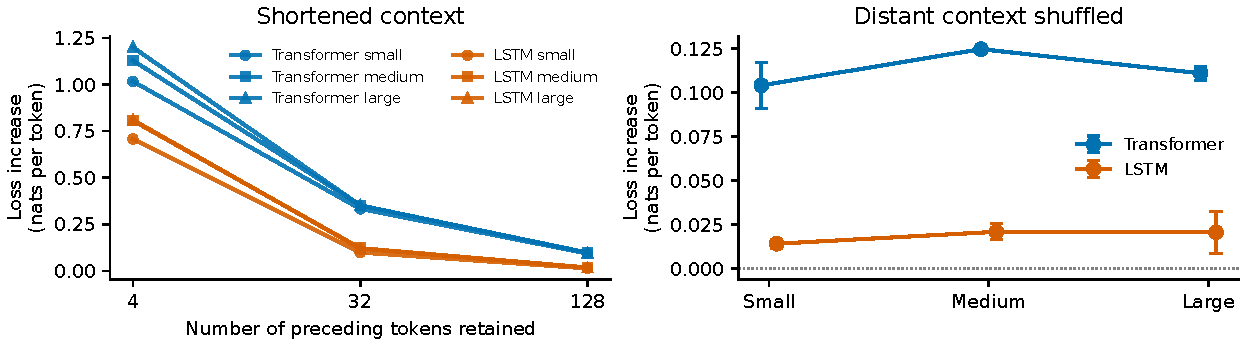
\includegraphics[width=0.93\linewidth]{figures/context_intervention.pdf}
\caption{Increase in prediction loss after shortening or shuffling context, relative to intact history. Each condition predicts the same 69,376 target tokens. The left panel averages three training repetitions; the right adds sample-standard-deviation error bars. Positive penalties indicate useful information in the removed or disrupted history. The 5-gram baseline has zero penalty throughout.}
\label{fig:context}
\end{figure}

\subsection{Copying is stronger than a generic second-span effect}

Repeating natural text favors Transformers by more than one nat per token at the main sequence length of 100. This far exceeds the 5-gram baseline's boundary effect. LSTM gains decline as sequences lengthen, consistent with difficulty preserving detailed token information throughout a long passage. Random-token repetition provides a complementary test: it reduces the usefulness of ordinary linguistic patterns and rewards recognizing the relation between first and second occurrences. Success on this task indicates sequence reuse rather than grammatical knowledge.

The contrast persists for 200-token natural-text sequences: repetition gain is 1.379 nats for the large Transformer versus 0.041 for the large LSTM. For 100-token random sequences, gains are 3.40, 6.18, and 6.62 for small, medium, and large Transformers, compared with 0.17, 0.25, and 0.18 for the corresponding LSTMs. These task-specific differences support a separation between repetition ability and grammatical judgments.

The independent-sequence control can show negative gain because unrelated text is harder to predict after another passage than the initial passage was after a sequence-start symbol. Subtracting that control answers a different question and does not replace the main repetition measure. Excluding the first four positions separately removes transitions that a 5-gram can exploit. These controls distinguish repetition-sensitive behavior from boundary effects, while the different sampled examples remain a limitation of cross-architecture repetition comparisons.

\subsection{Grammar scores do not follow the perplexity ranking}

Neural-model BLiMP accuracies cluster around 60--64\%, despite much larger differences in perplexity. This separation is weaker than a demonstration of grammar equivalence: a model may predict ordinary text better while judging particular grammatical contrasts less accurately. For medium models, LSTM subject--verb agreement accuracy is 68.63\% versus Transformer accuracy of 61.66\%, while licensing of negative-polarity expressions such as \emph{ever} is 37.17\% versus 44.29\%. For large models, Transformer determiner--noun agreement reaches 82.62\% versus 77.98\% for LSTM. These descriptive breakdowns show that a small overall difference can conceal opposing grammatical strengths.

A shared tokenizer does not eliminate differences between training and evaluation text. A question-mark token absent from WikiText training appears in eight BLiMP contrasts, sometimes only in the grammatical sentence. KenLM assigns unseen symbols its unknown-word probability; neural models can output every vocabulary token but have not learned this token from positive training targets. Excluding affected contrasts, matching sentence token counts, and averaging scores per token therefore change what is measured and must remain separate analyses. On equal-length pairs, accuracies are 58.69, 60.49, and 63.46\% for small, medium, and large Transformers, versus 62.91, 63.79, and 62.94\% for LSTMs. With scores averaged per token, the respective values are 57.58, 58.85, and 61.19\% versus 60.88, 61.51, and 60.86\%. The large Transformer's advantage shrinks in both analyses, showing that its grammar result depends partly on the scoring choice.

An error from the large Transformer trained with random seed 13 illustrates the problem. It assigns log probabilities $-100.90$ to ``Should the school ever collaborate?'' and $-64.36$ to ``The school should ever collaborate.'' It therefore favors the ungrammatical sentence, although the question licenses \emph{ever}. This example was selected as that model's most strongly preferred incorrect answer, not as a representative sample. Punctuation coverage and grammatical licensing both matter, so the scores do not isolate either cause. Corresponding sentence-level LSTM scores were unavailable, preventing a direct comparison of the two models on this example.

The uncertainty about equivalence is driven by training variation, not simply by the number of test sentences. Thousands of BLiMP pairs can estimate one model's accuracy precisely, but do not create additional independently trained models. With three repetitions, an unadjusted 90\% paired-$t$ interval has half-width $2.92s_d/\sqrt{3}$, where $s_d$ is the standard deviation of the paired accuracy differences. Observed standard deviations of 1.29--1.77 percentage points imply half-widths of 2.18--2.99 points, already exceeding the equivalence margin. Thus the experiment lacks sufficient precision to establish the proposed equivalence, even before accounting for nonzero mean differences.

\subsection{Depth and optimization constrain the architectural conclusion}

The four-layer medium LSTM does not close the gap. Its two completed runs yield mean test perplexity 54.89, worse than 44.57 for the two-layer medium LSTM; the third run fails early when gradient values become nonfinite. A separate lower-learning-rate experiment completes all three repetitions but gives perplexity 55.04. The available deeper models therefore do not recover the two-layer model's performance. However, holding parameter count fixed requires narrower hidden states, and the deeper model inherits settings chosen for the small two-layer model. This control does not establish that greater recurrent depth is always harmful or that independently optimized deeper models would fail.

A further control would compare models with equally good validation perplexity, separating context behavior from overall prediction quality. The retained weights selected by validation and saved at training end provide no same-size cross-architecture pair within the prespecified 1\% tolerance. Intermediate validation measurements do not recover the corresponding model weights, so that comparison cannot be reconstructed from training curves alone. The results at equal token exposure remain informative, but do not isolate context use at equal overall predictive quality.

\section{Limitations and Responsible Use}

Three independent training repetitions limit conclusions about equivalence and scaling. Resampling test examples cannot replace additional model training, and the failed depth-control run reduces evidence for that control. Separate batch-size and learning-rate experiments answer different questions and are not pooled with the main repetitions.

Matched parameters and tokens do not imply identical optimization or computation. Settings are selected at the smallest size using one tuning seed, and embedding initialization differs between families. The selected LSTM learning rate is the largest searched, leaving open whether a broader search would improve it. Experiments also ran on different machines. Shared preprocessing, tokenization, and population counts agree, but the available LSTM records do not permit independent verification of every historical data file. That verification limit does not demonstrate that the underlying data differ.

Early-to-late context gain combines startup effects, token difficulty, and useful history. Predicting fixed targets after context changes reduces that ambiguity but still alters token positions or distant lexical structure. The 512-token ceiling excludes document-scale memory, and different repetition samples further limit causal attribution. Results concern small Transformers and classic LSTMs whose memory restarts for each text segment, evaluated on English Wikipedia and BLiMP; they do not characterize modern recurrent variants or general human grammatical competence.

The retained train/test duplicate and Wikipedia's editorial biases limit generalization. BLiMP covers selected generated contrasts and includes length/rare-token artifacts. The models are research artifacts, not authoritative grammar judges or factual information sources. No new human-subject data were collected. Releases should preserve attribution, source terms, and documented model limitations.

\section{Conclusion}

Under matched parameter and training-token budgets, Transformers predict WikiText more accurately and show stronger context use and repetition gains. Holding the predicted tokens fixed supports this conclusion beyond a position curve: intact distant context benefits Transformers more, while a 5-gram is invariant. The evidence nevertheless establishes neither that long context explains most of the perplexity gap nor that distant-context gains grow monotonically with size.

The grammar comparison requires a different conclusion. Its gap changes direction with size, and similar overall accuracies do not establish equivalence within two percentage points. The evidence therefore supports stronger context use while leaving grammar equivalence and increasing advantage with scale unresolved. The most useful next steps are to evaluate both architectures on identical repeated sequences, train more independent models to improve equivalence-test precision, and retain intermediate model weights for comparisons at matched validation perplexity.

\section*{Team Contributions and Use of AI Tools}

Cao Pham Minh Dang contributed approximately 50\% of the project, developing the shared tokenizer, implementing and training the Transformers, and evaluating their predictions. Hugo Centeno Sanz contributed approximately 50\%, implementing the LSTM and 5-gram models and conducting their experiments and evaluations. Both contributed to the architectural comparison and report. OpenAI Codex assisted report organization, drafting, and inspection of sources and experimental evidence. Reported measurements were checked against recorded training settings and result summaries. Experiments used university computing resources and public datasets.

\section*{Reproducibility Statement}

The accompanying implementation includes data preparation, tokenization, model definitions, training and evaluation procedures, and machine-readable result summaries. Dataset versions, training settings, random seeds, and model identities are recorded. Code and model weights are provided through the \href{https://github.com/dangpmcao/NLP-Project}{project repository} and \href{https://huggingface.co/centenohugo/context-not-grammar}{model-weight repository}. Figures and tables can be regenerated from the saved summaries on a CPU. Full reproduction requires the model weights and a compatible GPU environment; the training times above exclude validation and evaluation overhead. Some individual LSTM and 5-gram predictions were unavailable for this report, limiting independent reconstruction of sentence-level error comparisons.

\label{lastmainpage}
\clearpage
\bibliographystyle{plain}
\bibliography{references}

\clearpage
\appendix
\section{Additional Results}

The tables below report every main training repetition, the exact parameter counts, and statistical comparisons. Each neural model is selected using validation loss. Random seed is listed separately from model size so that the three independent repetitions remain identifiable. Preliminary runs and additional batch-size or learning-rate experiments are not treated as extra repetitions of the main experiment.

\begin{table}[ht]
\centering
\small
\setlength{\tabcolsep}{3pt}
\begin{tabular}{lllrrrrrr}
\toprule
Model & Size & Seed & \shortstack{Test\\perplexity} & \shortstack{Grammar\\accuracy (\%)} & \shortstack{Context\\gain} & \shortstack{Repetition\\gain} & \shortstack{128-token\\penalty} & \shortstack{Shuffle\\penalty} \\
\midrule
Transformer & Small & 13 & 41.52 & 59.40 & 0.612 & 1.058 & 0.084 & 0.090 \\
Transformer & Small & 37 & 40.00 & 60.08 & 0.645 & 1.446 & 0.098 & 0.107 \\
Transformer & Small & 73 & 39.40 & 59.27 & 0.661 & 1.389 & 0.099 & 0.115 \\
LSTM & Small & 13 & 56.68 & 61.74 & 0.407 & 0.071 & 0.014 & 0.012 \\
LSTM & Small & 37 & 56.31 & 64.64 & 0.394 & 0.067 & 0.013 & 0.017 \\
LSTM & Small & 73 & 56.75 & 60.32 & 0.400 & 0.065 & 0.013 & 0.013 \\
\midrule
Transformer & Medium & 13 & 30.86 & 60.89 & 0.702 & 1.539 & 0.096 & 0.124 \\
Transformer & Medium & 37 & 30.79 & 62.18 & 0.690 & 1.582 & 0.099 & 0.124 \\
Transformer & Medium & 73 & 30.61 & 61.41 & 0.683 & 1.539 & 0.100 & 0.126 \\
LSTM & Medium & 13 & 44.16 & 62.36 & 0.453 & 0.095 & 0.019 & 0.022 \\
LSTM & Medium & 37 & 44.42 & 62.02 & 0.432 & 0.097 & 0.018 & 0.016 \\
LSTM & Medium & 73 & 45.12 & 64.54 & 0.438 & 0.096 & 0.018 & 0.025 \\
\midrule
Transformer & Large & 13 & 24.74 & 64.65 & 0.720 & 1.660 & 0.096 & 0.108 \\
Transformer & Large & 37 & 24.86 & 64.19 & 0.715 & 1.628 & 0.098 & 0.109 \\
Transformer & Large & 73 & 24.50 & 63.07 & 0.705 & 1.590 & 0.098 & 0.116 \\
LSTM & Large & 13 & 45.32 & 61.59 & 0.421 & 0.065 & 0.015 & 0.014 \\
LSTM & Large & 37 & 44.89 & 62.20 & 0.416 & 0.078 & 0.016 & 0.013 \\
LSTM & Large & 73 & 37.42 & 62.58 & 0.472 & 0.128 & 0.023 & 0.034 \\
\midrule
\bottomrule
\end{tabular}
\caption{Results for every main training repetition, with weights selected by validation loss. Grammar accuracy uses BLiMP; repetition gain uses 100-token natural-text sequences. The final columns show loss increases when context is limited to 128 tokens or when more distant tokens are shuffled. All gains and penalties use nats per token.}
\label{tab:seeds}
\end{table}

\begin{table}[ht]
\centering
\small
\begin{tabular}{lrrrr}
\toprule
Model and size & Other parameters & Token embeddings & Total & Completed runs \\
\midrule
Transformer, small & 3,290,624 & 4,194,304 & 7,484,928 & 3/3 \\
Transformer, medium & 10,844,160 & 6,291,456 & 17,135,616 & 3/3 \\
Transformer, large & 39,717,120 & 10,485,760 & 50,202,880 & 3/3 \\
LSTM, small & 3,285,376 & 4,194,304 & 7,479,680 & 3/3 \\
LSTM, medium & 10,836,060 & 6,291,456 & 17,127,516 & 3/3 \\
LSTM, large & 39,708,880 & 10,485,760 & 50,194,640 & 3/3 \\
LSTM, medium, four layers & 10,828,992 & 6,291,456 & 17,120,448 & 2/3 \\
\bottomrule
\end{tabular}
\caption{Exact parameter counts. Parameters other than token embeddings include learned Transformer positions and the LSTM output adapter. Only two of the three four-layer LSTM runs complete at the main learning rate; the separate lower-rate experiment completes all three.}
\label{tab:exactcounts}
\end{table}

\begin{table}[ht]
\centering
\small
\begin{tabular}{llrrr}
\toprule
Measure & Model size & \shortstack{Transformer\\minus LSTM} & 95\% interval & Adjusted $p$ \\
\midrule
Context gain (nats) & Small & 0.239 & $[0.164,0.313]$ & 0.01299 \\
Context gain (nats) & Medium & 0.251 & $[0.234,0.268]$ & 0.00073 \\
Context gain (nats) & Large & 0.277 & $[0.183,0.371]$ & 0.01299 \\
Grammar accuracy (points) & Small & -2.65 & $[-7.06,1.75]$ & 0.956 \\
Grammar accuracy (points) & Medium & -1.48 & $[-5.56,2.60]$ & 0.956 \\
Grammar accuracy (points) & Large & 1.85 & $[-1.37,5.06]$ & 0.956 \\
Change in context-gain gap & Large minus small & 0.038 & $[-0.115,0.191]$ & 0.396 \\
\bottomrule
\end{tabular}
\caption{Differences paired by training seed. Context-gain tests ask whether the Transformer advantage is positive and retain all six planned context/repetition comparisons in Holm correction. Grammar $p$-values test equivalence within two percentage points, with correction across sizes; their decisions use the 90\% intervals in the main text, not the descriptive 95\% intervals shown here. Scaling retains both planned comparisons. Withheld repetition tests receive conservative values of 1 only for adjustment. Intervals are not adjusted for multiple comparisons.}
\label{tab:inference}
\end{table}

\paragraph{Available evidence and reproduction limits.}
Recorded summaries provide per-model metrics, training settings, parameter counts, and identities of the weights used for evaluation. These support reconstruction of the aggregate comparisons above. Individual LSTM and 5-gram sentence predictions and some detailed evaluation outputs were unavailable for independent inspection. Recovering those outputs is necessary to reproduce individual cross-model disagreements or uncertainty analyses based on jointly resampling the same test examples. Aggregate summaries alone cannot reconstruct missing predictions or model weights.


\end{document}
